\section{Experimental Results}
\label{sec:results}
The experiments conducted in this study were designed to assess the effect of concept drift on the performance of the second proposed approach in detecting emerging new classes. The primary goal was to identify the machine learning algorithm in conjunction with DES, Dynamic Ensemble Selection technique, which improves the performance of classification when faced with the emergence of new classes. By conducting these experiments, valuable insights were gained, leading to potential enhancements in the effectiveness of the second proposed approach in managing imbalanced data streams and its overall performance. These experiments provide valuable insights into the capabilities of the framework and shed light on the optimal approach for handling emerging new classes in the presence of concept drift. The results provide valuable guidance for selecting the most suitable classification machine learning algorithm and DES configuration aims to enhance both classification performance and robustness. The experiments detailed in this study offer crucial insights into improving the second proposed approach's performance and tackling challenges related to emerging new classes and concept drifts in incremental drifted streams. These insights are instrumental in advancing stream mining techniques and developing more precise and resilient classification models for dynamic and evolving data-stream environments.
\subsection{Experimental Setup}
\label{sec:setup}
The evaluation of the second proposed approach involves a comparison with SENCForest \cite{mu2017classification}, SENNE \cite{yang2021concept}, and KENNES \cite{zhang2022knnens}. The evaluation utilizes several metrics, including recall, precision, F1 score \cite{sasaki2007truth}, BAC \cite{brodersen2010balanced}, and G-mean \cite{kubat1997addressing}. The procedure for experimentation followed a test-then-train technique \cite{krawczyk2017ensemble}, where the classifier is first trained on a specific chunk and then evaluated on the subsequent chunk. Each chunk was standardized to 2000 instances. Four different classification models served as base estimators: Gaussian Naive Bayes (GNB) technique, K-Nearest Neighbors (KNN), the Support Vector Classifier (SVC), and the Hoeffding Tree (HT), all features are implemented using scikit-learn \cite{ksieniewicz2022stream}. We establish an ensemble classifier pool with a set limit of L = 8, wherein each ensemble consists of N = 4 base models. While these constraints remained fixed across all experiments, the threshold for the pool classifier in each approach was maintained at eight. Consequently, if the threshold is surpassed, the least-performing classifier is systematically eliminated. ADWIN \cite{adams2023explainable} and DDM \cite{gama2004learning} are employed as concept drift detectors as implemented in the River library \footnote{\url{https://riverml.xyz/0.21.0/introduction/basic-concepts/}} , to identify concept drifts, as they are considered more accurate techniques for use in incremental data streams \cite{gama2004learning,adams2023explainable,madkour2023historical,baena2006early}. This configuration was applied consistently across all approaches to ensure fair engagement. The experiments were conducted using Python, and the source code is available publicly on GitHub \footnote{\url{https://github.com/Amadkour/transfer_learning_with_concept_drift.git}}.
\subsection{Data Streams}
\label{sec:data_stream}
In this section, the performance of the second Proposed Approach (PA2), was evaluated using several datasets, including synthetic data streams, a real-world application stream, and benchmark datasets. To conduct the evaluations, the stream-learn and River python libraries \cite{ksieniewicz2022stream} were used. As detailed in Table \ref{table:table_1}, the Covertype dataset stream is used as the benchmark dataset in the study. This dataset comprises 52 features, 7 classes, and a total of 581,010 instances. It serves as a standard benchmark dataset widely used in stream mining research. For the evaluation of real application streams, the Sensor stream dataset was utilized. This dataset includes 5 features, 58 classes, and 392,600 instances in total, reflecting a real-world application scenario. Synthetic dataset stream was generated using the scikit-learn Python package \cite{ksieniewicz2022stream}. This synthetic stream was generated to mimic data streams and assess the performance of the second proposed method. It included 10 features and four classes, divided into 200 chunks, each with a size of 2,000. The effectiveness of the second proposed method was rigorously assessed using these datasets along with a stream-learn library. This thorough evaluation offered important insights into how well the approach manages various types of data streams, encompassing benchmark datasets, synthetic data streams, and real-world application streams.

\begin{table}[H]
	\centering
	\caption{Summary of Dataset Characteristics Utilized in the PA2 Experimental.}
  \resizebox{\textwidth}{!}{
	\begin{tabular}{|l|c|c|c|c|}
	\hline
	\textbf{Data stream}     & \textbf{Features} & \textbf{Classes} & \textbf{Instances} & \textbf{Chunk Size} \\ \hline
	Sensor stream \footnote{\url{https://www.cse.fau.edu/~xqzhu/Stream/sensor.arff}}    & 5               & 58            & 392600            & 2000                \\ \hline
	Covertype stream\footnote{\url{http://archive.ics.uci.edu/dataset/31/covertype}.} & 52              & 7             & 581010            & 2000                \\ \hline
	Synthetic stream      & 10              & 4             & 200000            & 2000                \\ \hline
	\end{tabular}
  }

	\label{table:table_1}
	\end{table}

\subsection{Compared Approaches}
\label{sec:compared_approaches}
In the following section, a comparative analysis between GNB methodology and three established benchmark techniques is presented, detailed as follows:
\begin{enumerate}
	\item \textbf{SENCForest \cite{mu2017classification}:} The SENCForest method employs anomaly detection techniques to identify new classes and is founded on entirely random trees. It constructs isolation trees for both classification and detection by subsampling from each class, utilizing 20 random trees and a subsample size of 20. Although it can operate with incomplete or no label information, it frequently suffers from elevated false positive rates and suboptimal runtime efficiency in practical applications.
	\item \textbf{SENNE \cite{zhu2020semi}:} Utilizing a hypersphere ensemble mechanism, SENNE calculates scores to identify both new and known classes. It operates with a buffer capacity of 100 and sets a new class-score threshold of 0.5.
	\item \textbf{KENNES \cite{zhang2022knnens}:} The KNNENS method addresses the dual challenge of detecting new classes and classifying known classes within a unified framework. It was configured with a buffer size of 100 and a new class score threshold of 0.5.
\end{enumerate}



\subsection{Examination of Experimental Findings}
\label{sec:finding}
This section offers an in-depth analysis of the second approach's performance across various data streams. To ensure a thorough evaluation, five performance metrics— recall, F1 score, precision, recall, G-mean, and BAG—are displayed through two types of visual diagrams: radar and line charts. The radar chart effectively summarizes the performance of each algorithm by highlighting their performance across the six key metrics. Additionally, to evaluate the overall performance of each method—including PA2, SENCForest, SENNE, and KENNES—the average value for each metric was computed. Additionally, a line diagram using the G-mean metric was used to compare these methods for each chunk across 200 chunks. A radar diagram provided a detailed and nuanced evaluation of the second approach’s performance across various experimental scenarios.

\subsubsection{Results On The Benchmark Dataset}
\label{sec:covertype}
\begin{figure}[H]
	\centering
	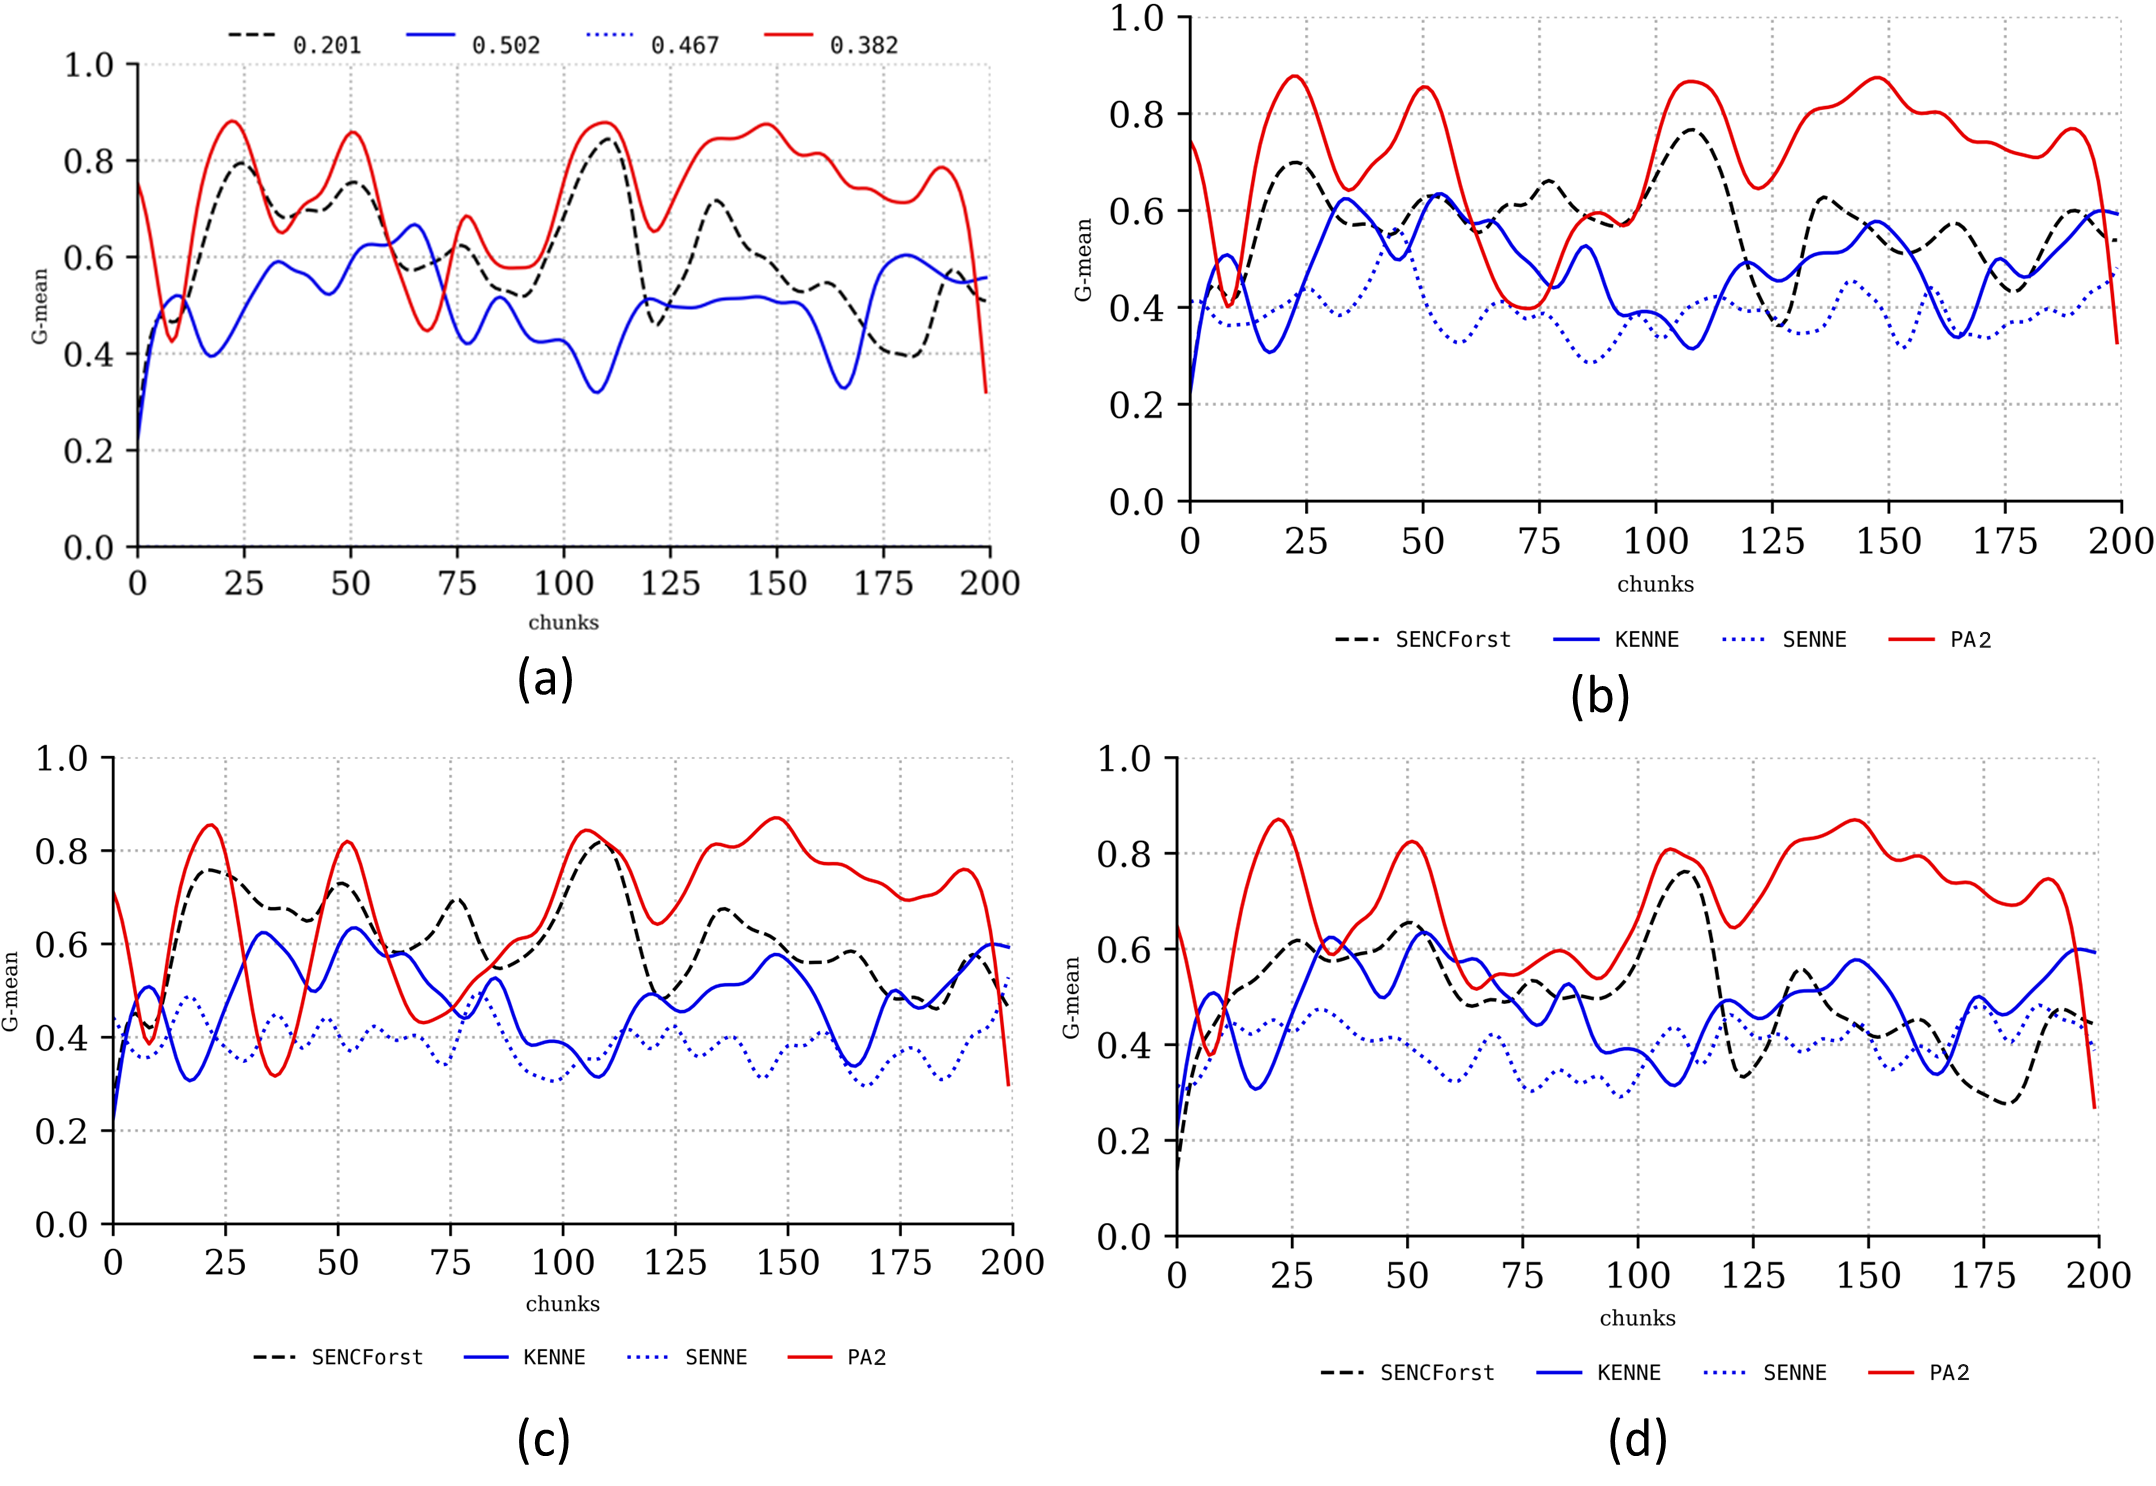
\includegraphics[width=1\linewidth]{5_Emerging/images/res1.png}
	\caption{Covertype Stream Performance.}

	\label{fig:res1}
\end{figure}
This experiment sought to evaluate the performance of the second approach on the Covertype data stream using different buffer sizes, with ADWIN employed as the concept drift detector. From a philosophical perspective, this experiment exemplifies the idea of adaptation to context and the gradual refinement of understanding. The experiment's findings are presented through scatter (line) plots in Figure \ref{fig:res1}, which depict the effects of emerging buffer sizes—5, 10, 20, and adaptive sizes—on performance. In the initial analysis (Fig. \ref{fig:res1}(b)), the G-mean of various methods—SENCForest, SENNE, KENNES, and PA2—across 200 chunks with a buffer size of 5 instances reveals that early performance is suboptimal. This initial period of underperformance mirrors philosophical concepts of learning through trial and error and the necessity of time for refinement. Similar to how human cognition or understanding improves after prolonged exposure to data or experience, the classifier pool grows in the experiment, which gradually enhances performance.  By chunk 20, the classifiers begin to adapt, as the dynamic ensemble selection (DES) technique can more effectively identify the most competent classifiers for future chunks. This process of selection reflects the philosophical notion of wisdom through discernment, where the system, like an informed agent, selects the best approach to navigate complexities. The performance improvements are particularly evident after chunk 20, with PA2 consistently outperforming other methods, while KENNES and SENNE lag behind, representing thediffering capacities of systems to adapt to and learn from new information.

The experiments with buffer sizes of 10 and 20 (Fig. \ref{fig:res1}(b) and Fig. \ref{fig:res1}(c)) show that while performance slightly decreases compared to the buffer size of 5, the larger buffer sizes may offer fewer opportunities for updates, illustrating the tension between stability and flexibility in knowledge systems. The adaptive buffer size experiment (Fig. \ref{fig:res1}(d)) further underscores the concept of continuous adaptation, where PA2’s superior performance highlights the algorithm’s ability to adjust dynamically to the data stream, providing the best outcomes across all chunks. The experiment reflects philosophical ideas of progressive refinement and adaptive responsiveness. Just as knowledge systems evolve by selecting the most relevant information at the right time, the classifier system's ability to choose the most effective classifiers through dynamic adaptation mirrors this ongoing process of learning and improvement.				

\subsubsection{Results On Real Application Stream}
\label{sec:sensor}
This experiment aimed to evaluate the performance of the algorithms SENCForest, SENNE, KENNES, and PA2 across 200 chunks of a sensor data stream, using varying buffer sizes similar to the previous experiment. The results, presented in Figure \ref{fig:res2}, are visualized through scatter plots. In Figure \ref{fig:res2}(a), the classification performance of each algorithm is shown with a buffer size of 5. The PA2 algorithm outperformed the others overall, except in chunks 43 to 48, where some instances were mistakenly identified as outliers instead of emerging classes. In contrast, SENCForest and SENNE exhibited the lowest performance. Further experiments with buffer sizes of 10 and 20 (Figures \ref{fig:res2}(b) and \ref{fig:res2}(c)) revealed a decline in performance compared to the buffer size of 5, likely due to fewer updates resulting from the larger buffer sizes. The adaptive buffer size experiment in Figure \ref{fig:res2}(d) reinforced the effectiveness of the PA2 algorithm, which consistently outperformed the other algorithms across all chunks, with the adaptive emerging pool size delivering the best results.
From a philosophical perspective, this experiment highlights the importance of dynamic adaptability in response to changing data, as well as the trade-off between stability and flexibility. The PA2 algorithm’s ability to adjust its performance through varying buffer sizes can be seen as an example of how systems of thought and knowledge can evolve by learning from emergent patterns and refining their strategies over time. The experiment underscores the balance between responsiveness and efficiency, suggesting that continuous adaptation can lead to more effective problem-solving and decision-making in dynamic environments.

\begin{figure}[!ht]
	\centering
	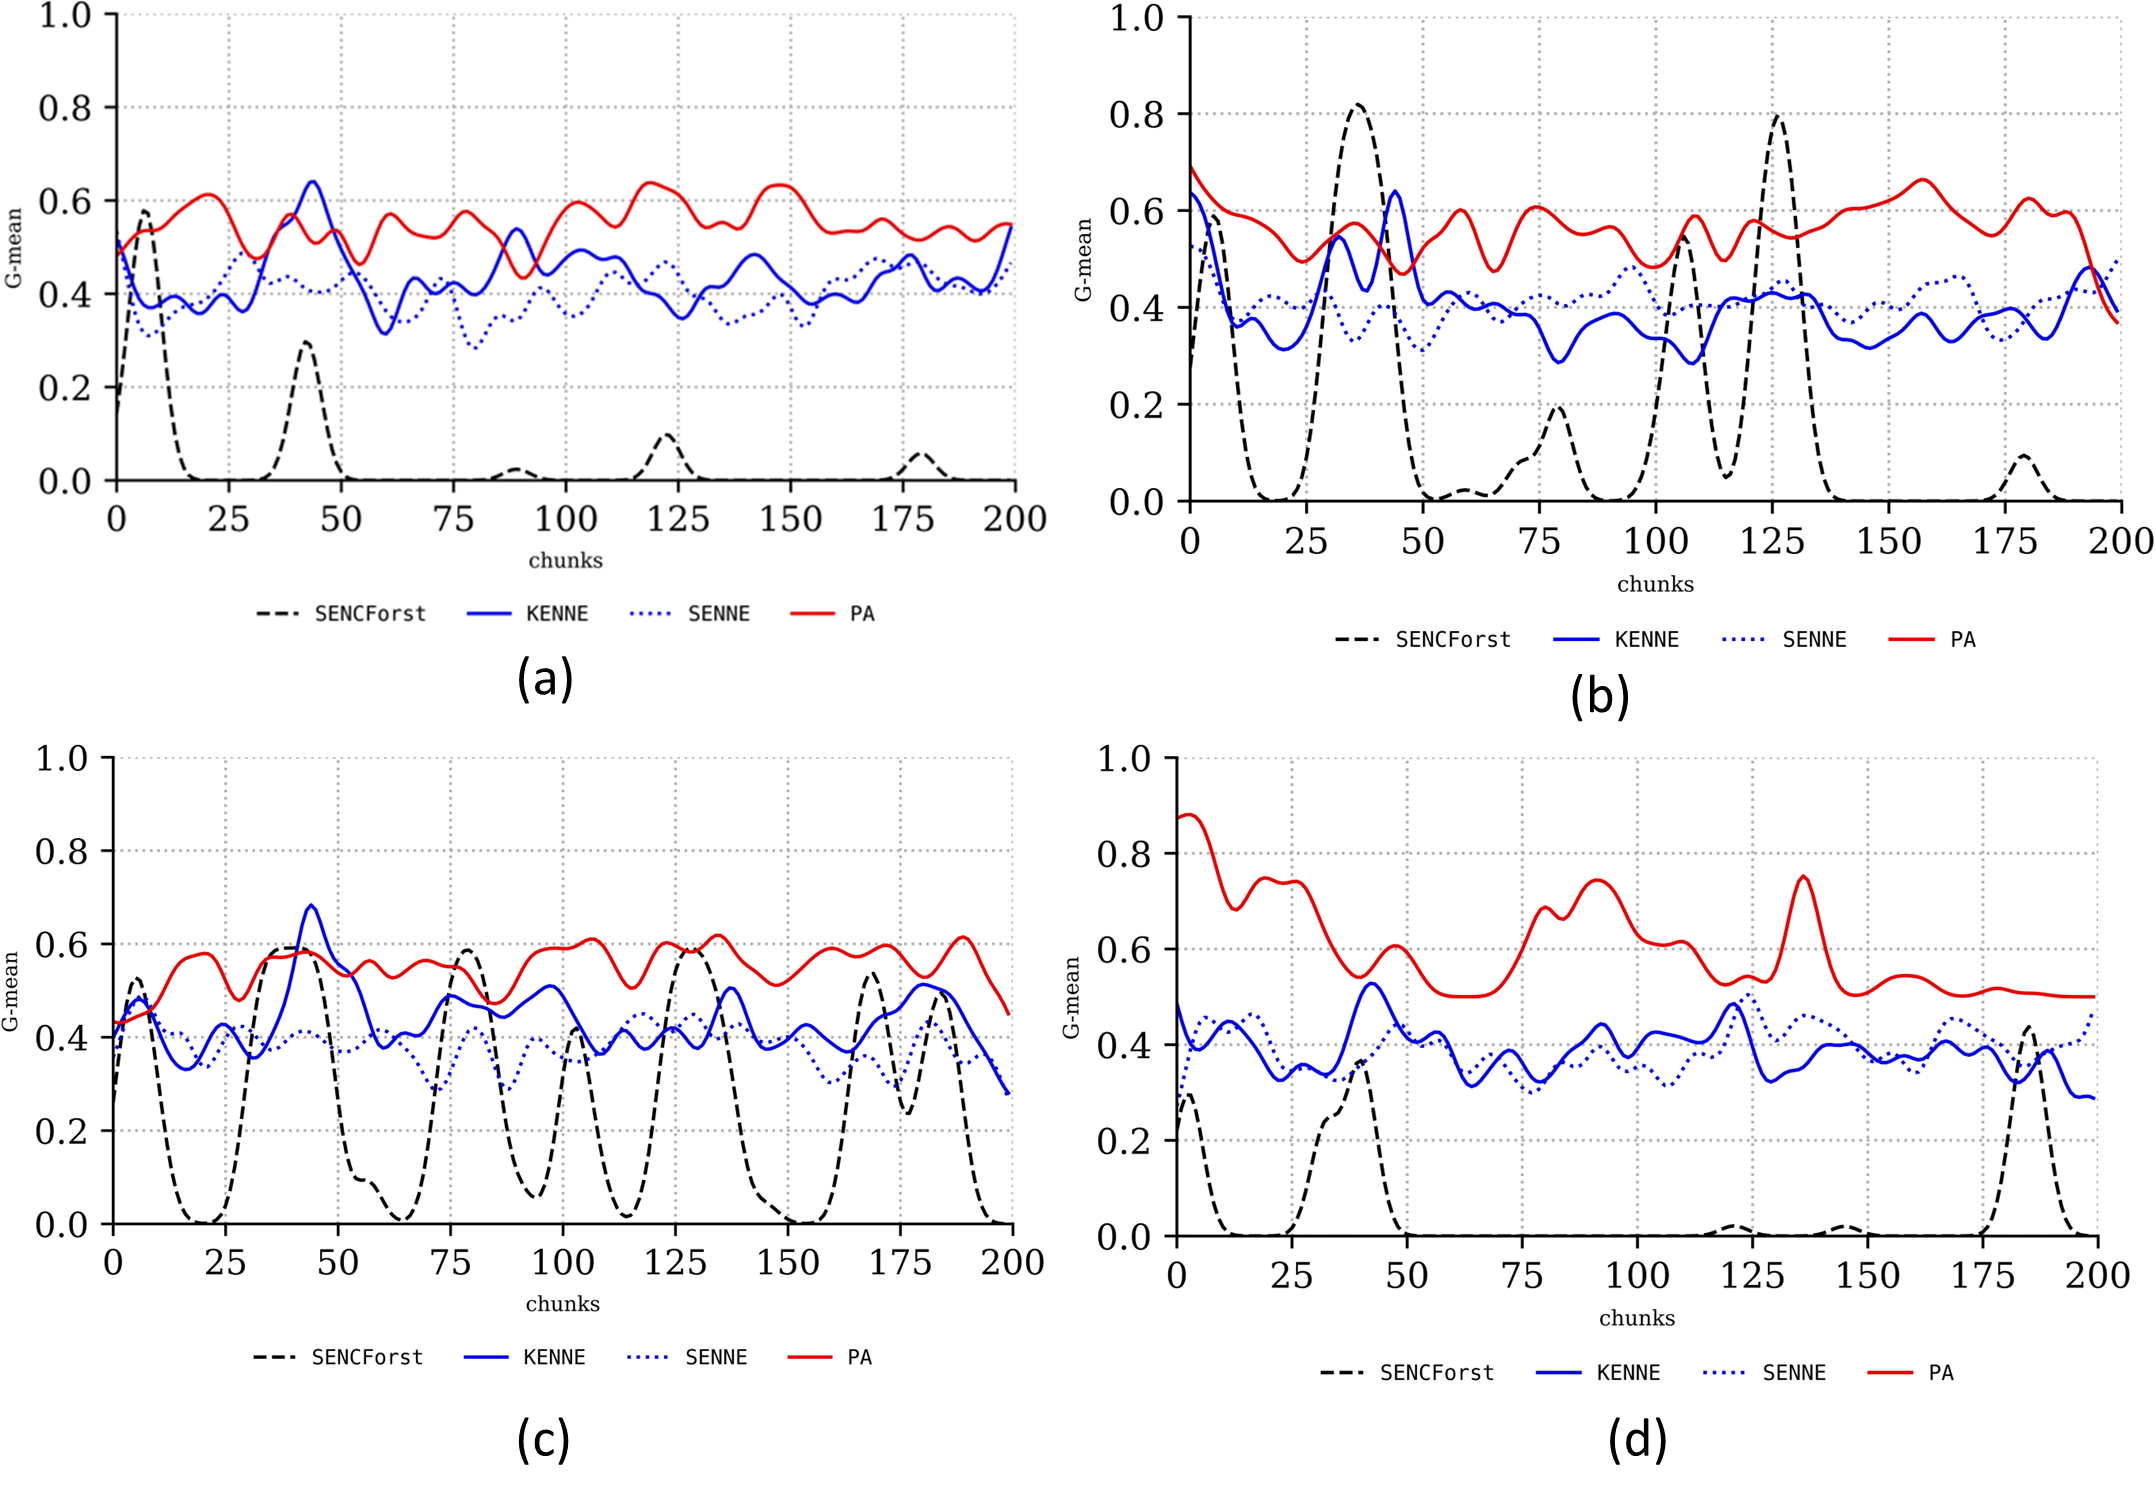
\includegraphics[width=1\linewidth]{5_Emerging/images/res2.png}
	\caption{Sensor Stream Performance.}

	\label{fig:res2}
\end{figure}				

\subsubsection{Results On Synthetic Stream}
\label{sec:synthetic}
This experiment sought to evaluate the performance of previously tested methods on a synthetic data stream. The results, presented in Figure \ref{fig:res3}, illustrate that the PA2 algorithm consistently achieved the highest performance across different buffer sizes of 5, 10, and 20. As shown in Figures \ref{fig:res3}(a), \ref{fig:res3}(b), and \ref{fig:res3}(c), scatter plots reveal PA2's superior performance in all these scenarios. Furthermore, Figure \ref{fig:res3}(d) highlights that the adaptive pool size yielded the best results on the synthetic stream, emphasizing the adaptive nature and efficiency of the PA2 algorithm.
Philosophically, this experiment underscores the importance of adaptability in complex and dynamic environments. The PA2 algorithm’s consistent superior performance reflects a system's ability to respond flexibly to emerging patterns and changing conditions, embodying the notion that the most effective strategies are often those that can continuously refine and adjust based on new information. This adaptability mirrors the process of philosophical growth, where knowledge systems must remain open to revision and improvement in response to evolving contexts, leading to more refined and robust outcomes over time.

\begin{figure}[!ht]
	\centering
	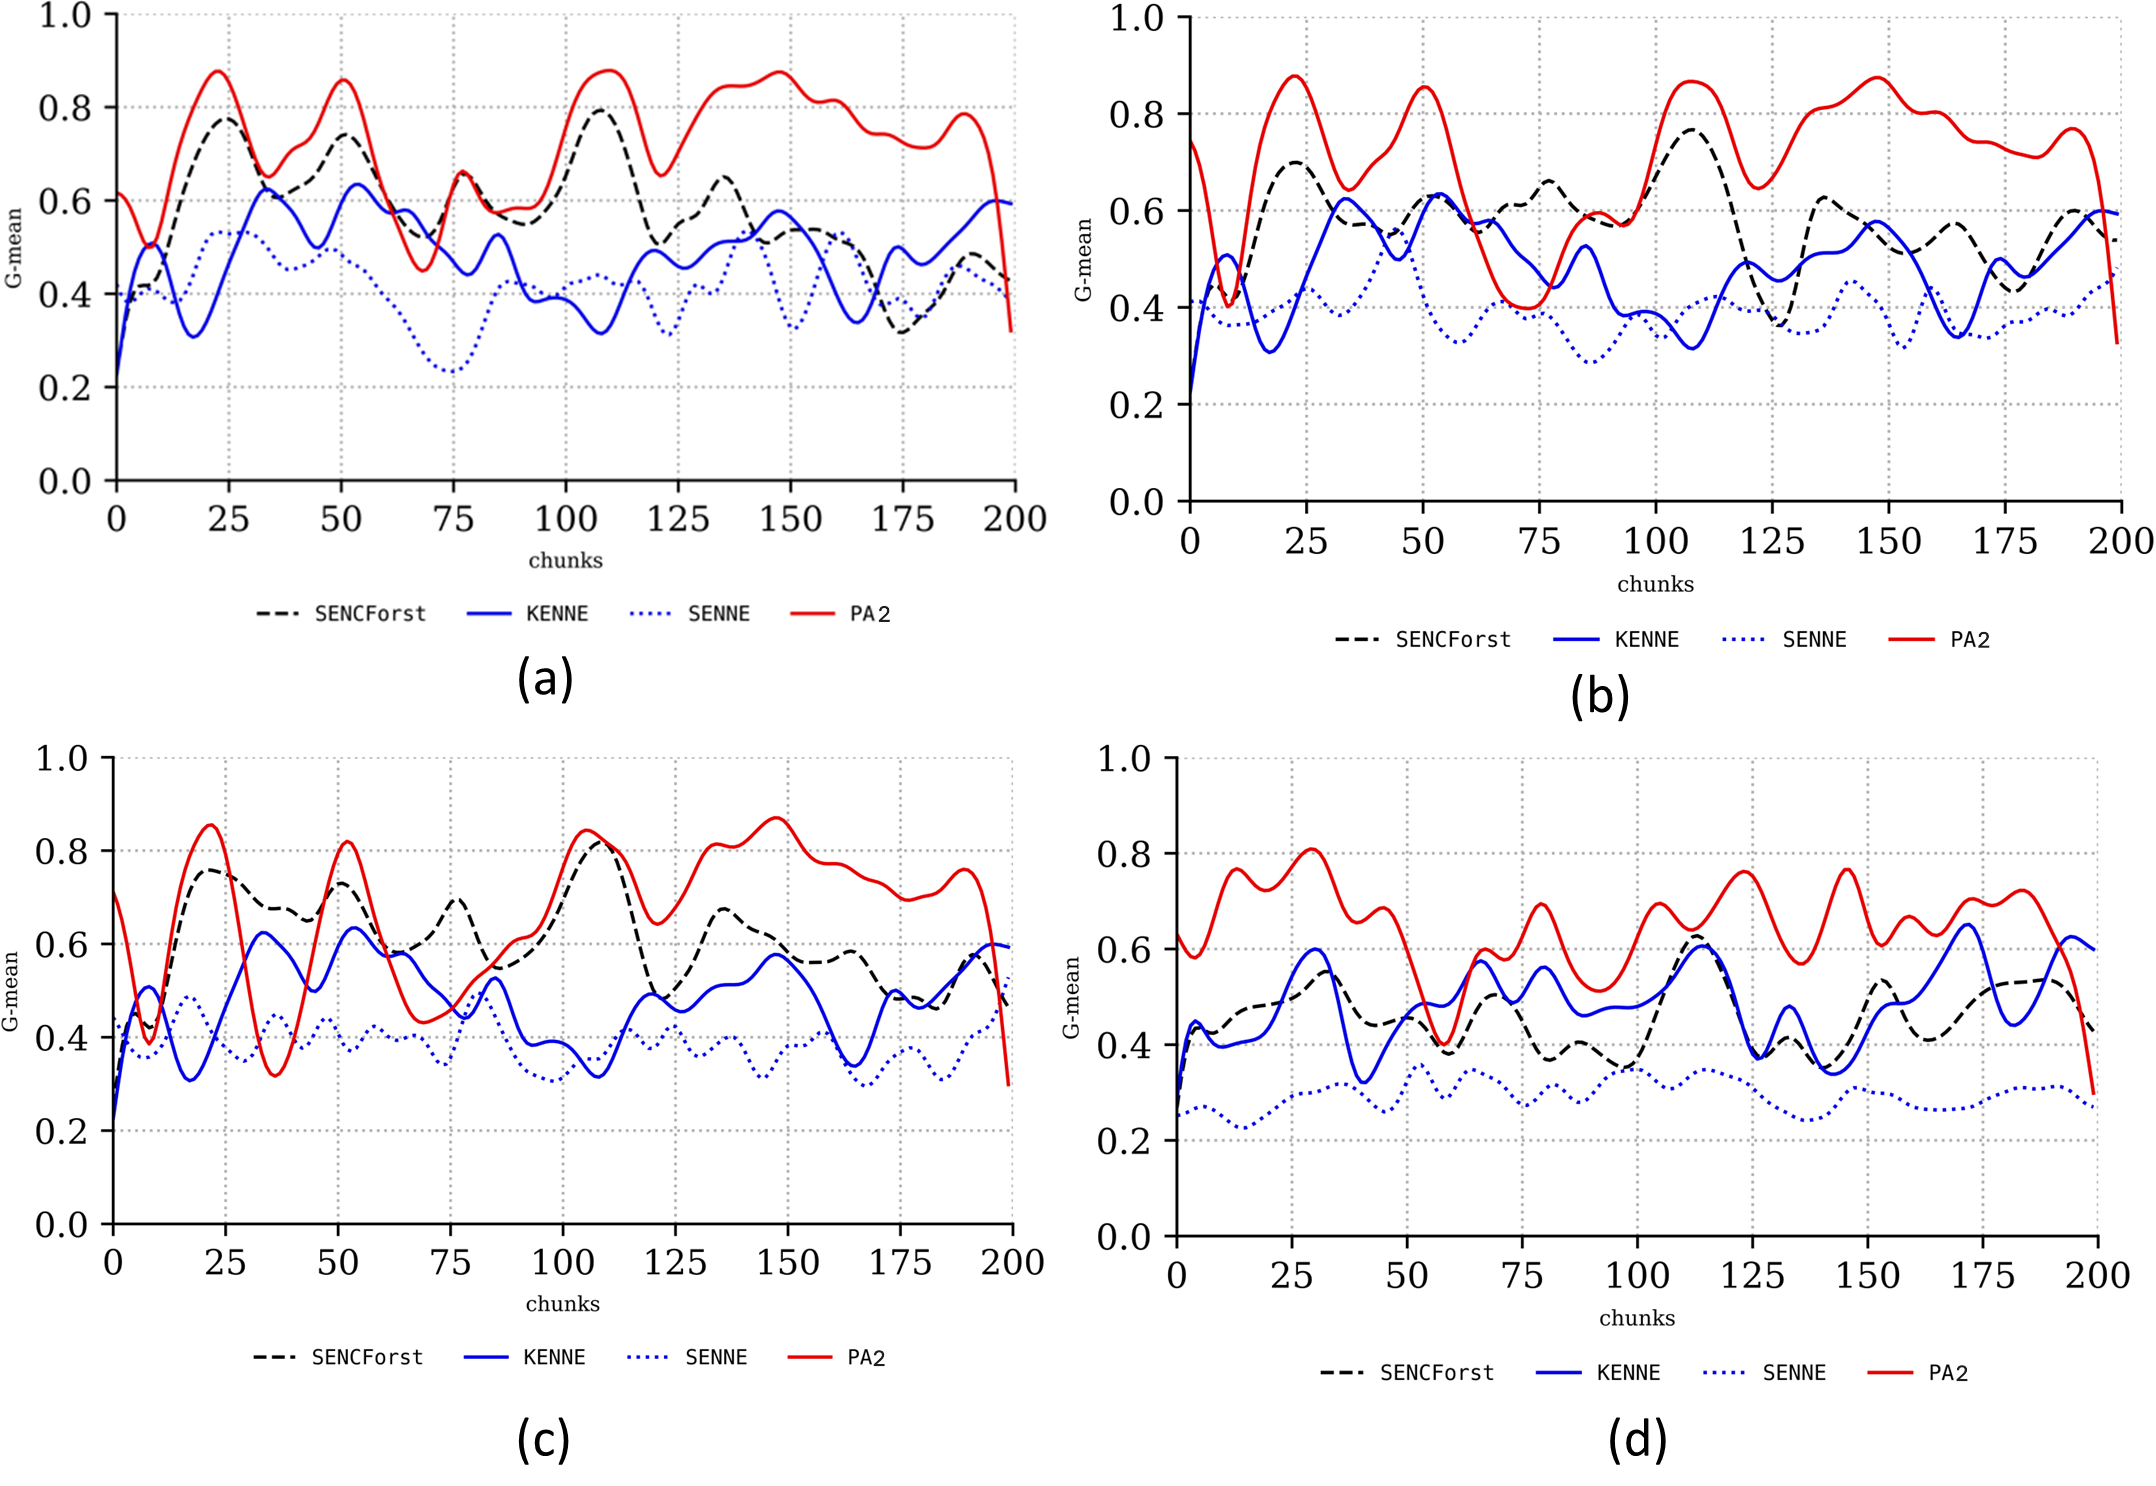
\includegraphics[width=1\linewidth]{5_Emerging/images/res3.png}
	\caption{Synthetic Stream Performance.}

	\label{fig:res3}
\end{figure}				

\subsection{Runtime Analysis Of The Best Algorithms}
\label{sec:running}
Our experimental results indicate that the selection of the optimal algorithm for detecting emerging new classes is influenced by several factors, including dataset characteristics, buffer length, and the algorithm's runtime requirements. A series of experiments were conducted to evaluate the runtime performance of different algorithms, with the PA2 algorithm demonstrating exceptional efficiency. Specifically, using the adaptive pool size approach, the PA2 algorithm trained bagging classifiers 150 times within 2131 seconds on the Covertype stream, outperforming others despite SENCForest achieving the lowest runtime but with fewer updates compared to PA2, as shown in Table \ref{table:table_2}. On the Sensor stream, PA2 delivered the best runtime for 66 updates, while SENCForest, KENNES, and SENNE required more time to complete the same or fewer iterations. Similarly, PA2 exhibited superior runtime performance on the Synthetic stream. These results underscore the PA2 algorithm’s efficiency, making it an ideal choice for time-constrained scenarios. The superior runtime performance of PA2 is further highlighted in bold in Table \ref{table:table_2}. These findings reflect the notion of pragmatic efficiency—the ability to achieve desired outcomes with optimal resource utilization. In decision-making and knowledge systems, the most effective strategies are often those that can maximize results while minimizing costs, both in terms of time and computational resources. The PA2 algorithm’s ability to consistently perform well under time constraints mirrors the importance of practical adaptability in real-world applications, where solutions must be both effective and efficient, capable of meeting demands without unnecessary complexity.
	
\begin{table}[t]
	\centering
	\caption{Runtimes (in seconds) Comparison of SENCForest, SENNE, KENNE, and PA2.}
  \resizebox{\textwidth}{!}{
	\begin{tabular}{|l|l|c|c|}
	\hline
	\textbf{Stream}    & \textbf{Algorithm} & \textbf{Training Times} & \textbf{Time (seconds)} \\ \hline
	Covertype          & SENCForest         & 142                     & \textbf{1997}           \\ \cline{2-4} 
					   & SENNE              & 5                       & 2167                    \\ \cline{2-4} 
					   & KENNES             & 3                       & 1742                    \\ \cline{2-4} 
					   & PA2                 & 150                     & 2131                    \\ \hline
	Sensor             & SENCForest         & 23                      & 1244                    \\ \cline{2-4} 
					   & SENNE              & 17                      & 3825                    \\ \cline{2-4} 
					   & KENNES             & 152                     & 2109                    \\ \cline{2-4} 
					   & PA2                 & 66                      & \textbf{1075}           \\ \hline
	Synthetic          & SENCForest         & 12                      & 107                     \\ \cline{2-4} 
					   & SENNE              & 26                      & 224                     \\ \cline{2-4} 
					   & KENNES             & 149                     & 202                     \\ \cline{2-4} 
					   & PA2                 & 47                      & \textbf{91}             \\ \hline
	\end{tabular}
  }

	\label{table:table_2}
	\end{table}

\subsection{Comparison between GNB, KNN, and HT, SVC}
\label{sec:compared_base_calssfier}
In this section, a comparison of various algorithms—KNN, SVC, GNB, and HT—was conducted as base classifiers for the bagging technique. This comparison, shown in Figure \ref{fig:res4}, focuses on the Covertype dataset stream, where GNB (blue line) and HT (red line) consistently achieved the highest scores across most chunks. Both classifiers also performed well in radar plots across key performance metrics, such as balanced accuracy, precision, recall, G-mean, and F1 score. Based on these results, GNB and HT were identified as the most suitable base classifiers for the bagging technique. Further comparisons between GNB and HT in terms of runtime and update frequency, as presented in Table \ref{table:table_3}, revealed that GNB offers the best runtime performance. However, HT demonstrated superior overall performance, likely due to its higher number of updates compared to GNB, as reflected in Table \ref{table:table_3} and Figure \ref{fig:res4}. This analysis touches on the concept of trade-offs in decision-making and the balancing of multiple objectives. In this case, the trade-off between runtime efficiency (GNB) and performance improvement through frequent updates (HT) mirrors the broader challenge of optimizing strategies in real-world scenarios. The findings suggest that different approaches are suitable for different goals, with GNB excelling in time-sensitive contexts, while HT performs better when frequent adjustments and continuous learning are prioritized. This reflects the broader philosophical notion that optimality is context-dependent, and the best solution often depends on the specific demands of the environment or problem at hand.

\begin{figure}[t]
	\centering
	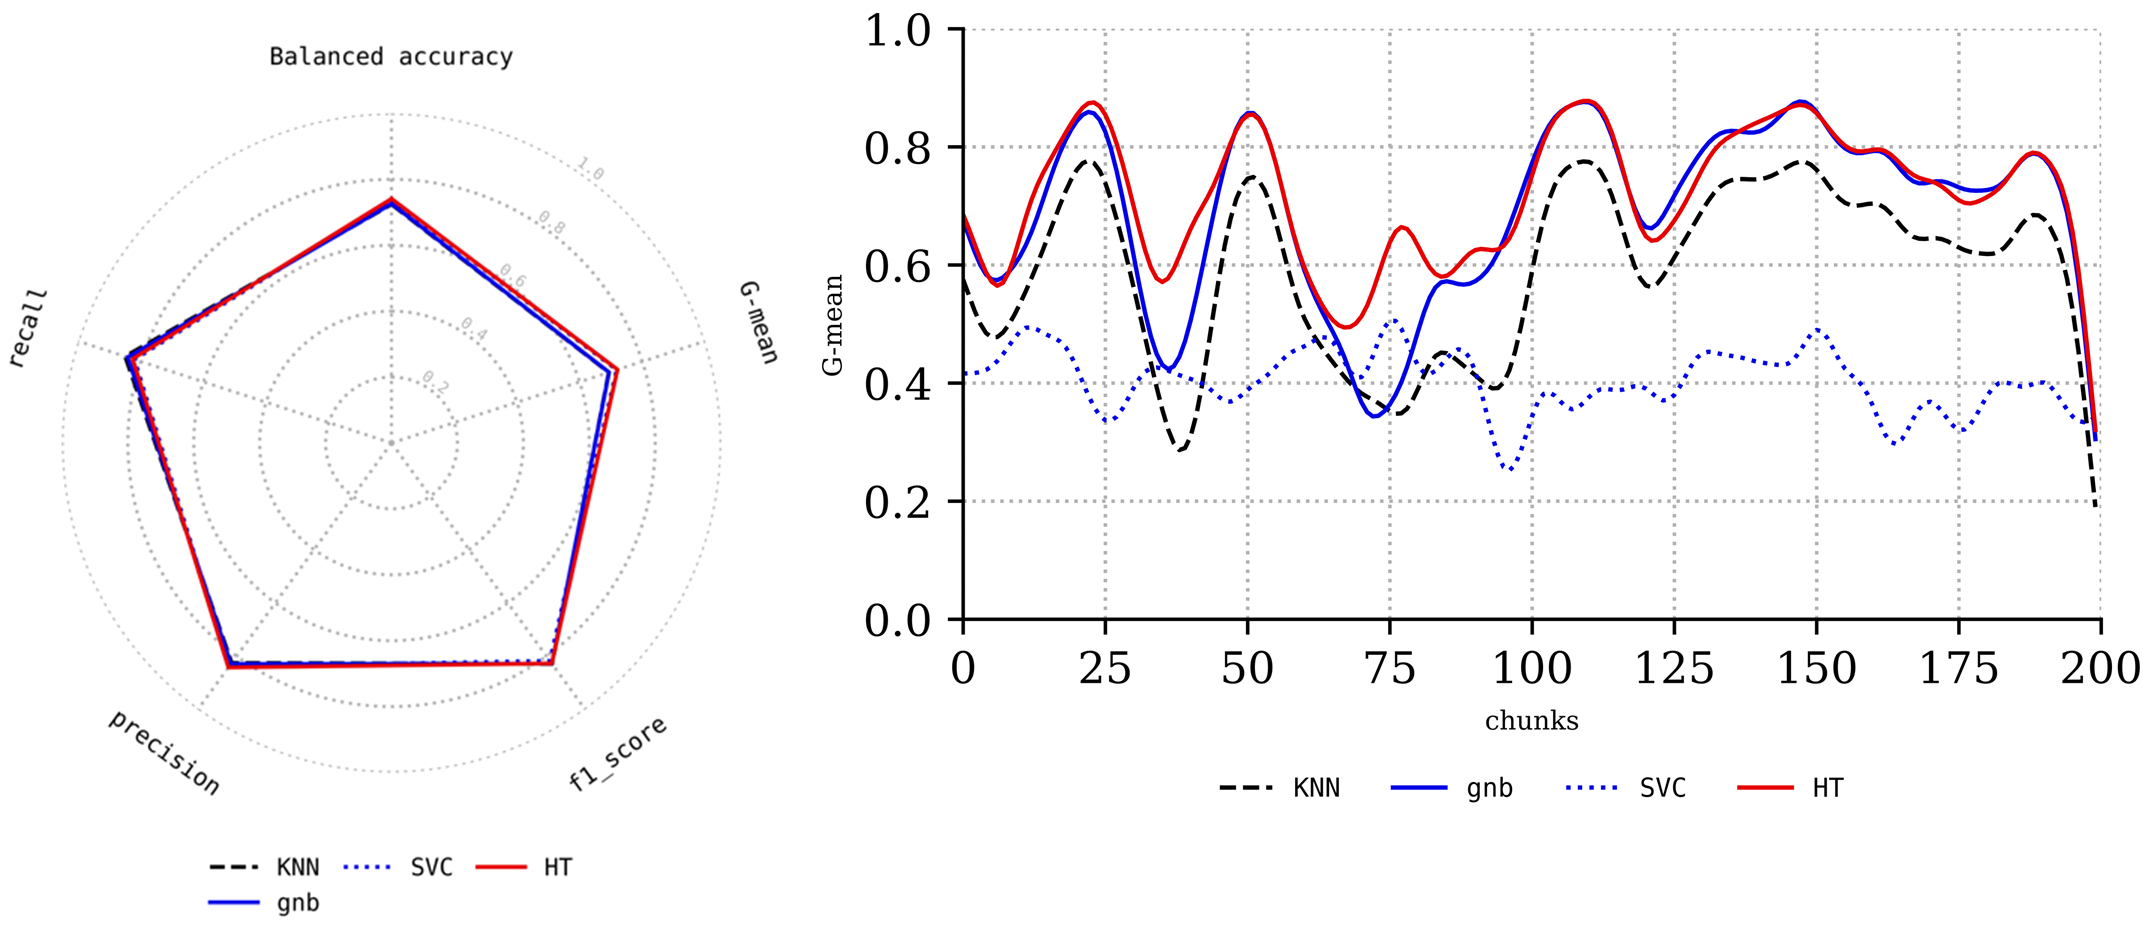
\includegraphics[width=1\linewidth]{5_Emerging/images/res4.png}
	\caption{Performance Metrics for Covertype Stream with ADWIN and DDM.}

	\label{fig:res4}
\end{figure}				

	
\begin{table}[t]
	\centering
	\caption{Runtimes (in seconds) of KNN, SVC, GNB, and HT.}
	\begin{tabular}{|l|c|c|c|c|}
	\hline
	\textbf{Algorithm}     & \textbf{KNN} & \textbf{SVC} & \textbf{GNB} & \textbf{HT} \\ \hline
		Training Times         & 140          & 150          & \textbf{139} & 148         \\ \hline
		Runtimes (in seconds)         & 586          & 878          & \textbf{291} & 1169        \\ \hline
	\end{tabular}
	\label{table:table_3}
	\end{table}


\subsection{Comparison between ADWIN and DDM}
\label{sec:compared_drift_detector}
In this section, two concept drift detection methods, the Drift Detection Method (DDM) \cite{gama2004learning} and the Adaptive Window (ADWIN) \cite{gama2004learning, adams2023explainable}, are compared. Both methods are highly regarded for their performance in managing incremental drifted streams \cite{gama2004learning, adams2023explainable, madkour2023historical, baena2006early}. Figure \ref{fig:res5} illustrates that when using the Synthetic stream with GNB as the base classifier, ADWIN consistently outperforms DDM in both radar and line plots across all performance metrics, including G-mean. Additionally, a comparison of their runtime and update frequency, shown in Table \ref{table:table_4}, reveals that ADWIN is the superior drift detector. It identifies the highest number of drifts (139) in the least amount of time (272 seconds), demonstrating its efficiency and effectiveness. This comparison highlights the concept of efficiency versus accuracy in decision-making. ADWIN's superior performance can be interpreted as a reflection of adaptive learning—the ability to respond swiftly and effectively to changes in data, a key aspect of systems designed for dynamic environments. This adaptability mirrors the philosophical idea of pragmatism, where the best solution is not necessarily the most static or fixed but one that evolves in response to changing circumstances. In the context of concept drift, the ability to efficiently identify and react to changes is crucial, suggesting that dynamic systems that can self-adjust are often more effective than those that require fixed, predefined responses.
\begin{figure}[!ht]
	\centering
	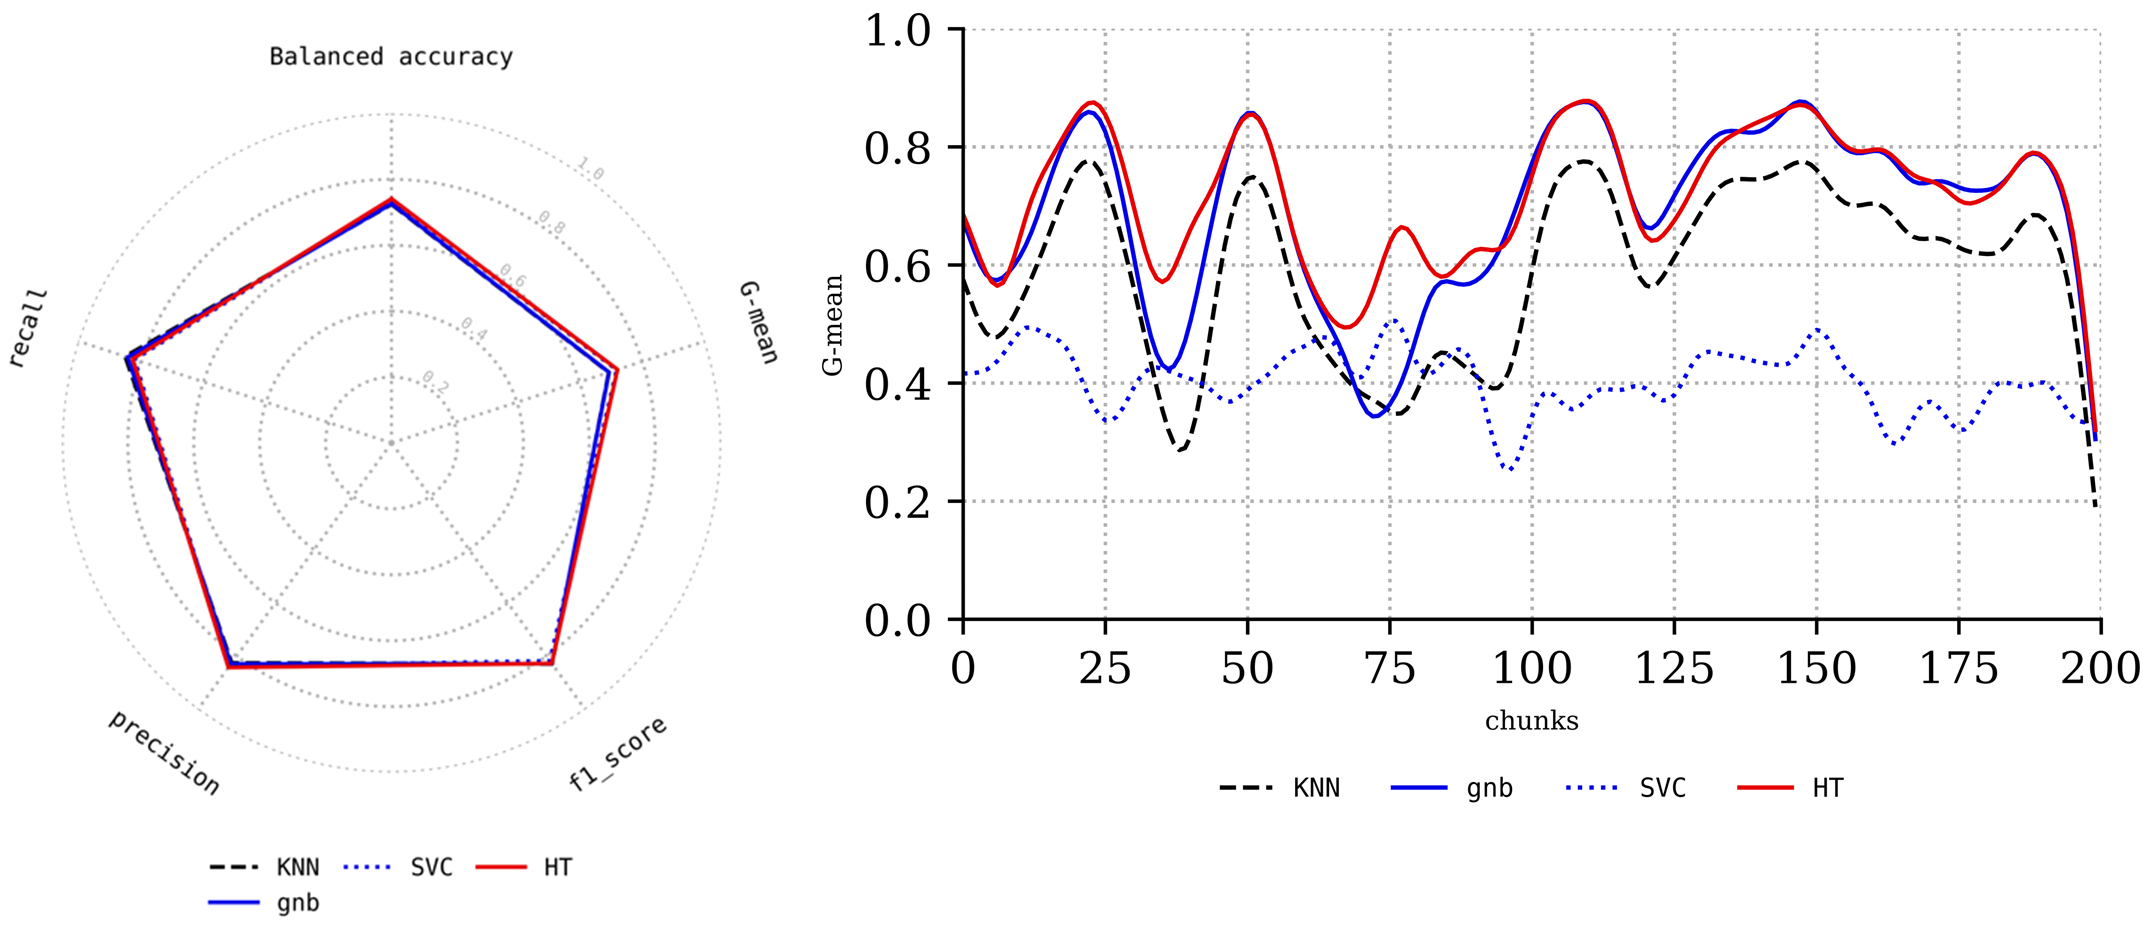
\includegraphics[width=1\linewidth]{5_Emerging/images/res4.png}
	\caption{Performance Metrics for Synthetic Stream with ADWIN and DDM.}

	\label{fig:res5}
\end{figure}
	
\begin{table}[!ht]
	\centering
	\caption{Runtimes (in seconds) of ADWIN and DDM.}
	\begin{tabular}{|l|c|c|}
		\hline
	\textbf{Algorithm}     & \textbf{ADWIN} & \textbf{DDM}  \\ \hline
Training Times         & 139          & 55                   \\ \hline
Runtimes (in seconds)         & 272          & 545                   \\ \hline
	
	\end{tabular}
	\label{table:table_4}
	\end{table}